%!TEX root = ../thesis.tex
%*******************************************************************************
%****************************** Third Chapter **********************************
%*******************************************************************************
\chapter{Scene Surveying}\label{chapter:SceneSurveying}
In this chapter, we provide details of the techniques and software developed to address the problem of aiding autonomous scene surveying, which was identified as part of the first research question stated in Section \ref{sec:ResearchQuestions}: 
\\
\\
"\textit{Can an agent-based software system be developed to run on a system of heterogeneous autonomous aerial vehicles to aid the tasks of scene surveying and target localisation in a hazardous environment? }".
\\
\par As with the rest of the work in this thesis, this chapter is motivated by the context of the ROCSAFE project, but we present the work in a general setting. In the initial phase of any crime scene investigation, it is desirable for the crime scene manager to visually scan the entire crime scene area to thoroughly assess the scene as early as possible \cite{TechnicalWorkingGrouponCrimeSceneInvestigation2013CrimeEnforcement}. We will henceforth refer to the area to be scanned as the \textit{region of interest} for the purpose of generality. In the ROCSAFE project, it is intended to address this problem using a fleet of RAVs, which are equipped with cameras and sensors which are highly suited to data-gathering. The RAVs can operate concurrently and can communicate with a centralised controller. We developed a system to autonomously survey a hazardous situation using the simulation environment described in Chapter \ref{chap:HighFidelitySim}. We published this work in a number of papers \cite{Smyth2018AInvestigation}, \cite{Smyth2018ASupport}, \cite{Smyth2018UsingDrones}.
%The information acquired by this initial sweep can be used for a multitude of purposes and generally speaking the sooner it can be gathered, the better, since it will often be subjected to time-consuming analysis. 
%We used the simulation environment described in Section \ref{chap:HighFidelitySim} to test the developed system.
%In order to ensure that the solutions explored are not domain-specific, we make few assumptions regarding the nature of the hardware used to solve the problem. 
\par We began by providing a description of the two main sub-problems identified as part of autonomous scene-surveying:
\begin{enumerate}
    \item Given a polygonal region defined by a set of points that lie on the earth's surface, generate a discrete set of cells of uniform area that partition the region of interest.
    %according to a user-specified height and width. 
    The cells can be described by their center points, as they are assumed to be of uniform height and width. We will refer to this set as $R$, the set of \textit{waypoints}.
    \item Find a set of routes for each of $K$ RAVs to be used in the data-gathering process, such that these sets partition $R$ and the cost of the system of RAVs traversing these points is minimized. %Objective functions which define the cost of traversal are discussed in <reference relevant section>.
\end{enumerate}

Hence there are two main goals: find a discrete representation of a continuous area which represents the region of interest, and then find routes that the RAVs can execute in order to visit each of the grid points exactly once, while minimising the cost of doing so. 
%We then give a mathematical definition of the sub-problems in sections \ref{sec:GenerationOfWaypoints}, \ref{subsec:SimplifiedVRP} and \ref{sec:SceneSurveyingBatteryConstraints}.


\nomenclature[]{GPS}{Global Positioning System}
\nomenclature[]{WGS84}{World Geodetic System 1984}

\section{Generation of Waypoints}
We first address the issue of finding a discrete set of waypoints, referenced above as $R$. We chose to formulate the problem using a discrete set of waypoints, rather than deal with the case of treating the region as continuous space, since it is much easier to accurately record sensor data when the UAV has settled at a given point. Discretising the space also allows the problem to be formulated in a manner that is easier to tackle, without losing the key aspects.
%\begin{itemize}
    %\item It is more straightforward to describe the problem using a discrete set of points rather than a continuous one.
%    \item It is much easier to process sensor information if it is known exactly where this data has been captured. The UAVs may stop at each discrete waypoint to visit these locations. *Focus on this point, expand if possible*
%    \item The case of path-finding using discrete waypoints has a strong body of literature behind it
%    \item The UAVs run autopilot software which can guide them using the on-board GPS sensor
%\end{itemize}

%which are the center points of cells that partition the region of interest.
\note{set of waypoints create a voronoi partition, might be worth talking about}

\note{Above needs revision, will come back once rest of chapter has been fleshed out a bit more}
We began by assuming that the region which is to be surveyed, the \textit{region of interest}, can be described by a polygon on the x-y plane, since it allows for a discrete representation. We favour a discrete representation for the sake of simplicity, since it is computationally much easier to record and manipulate a set of points to represent the boundary rather than a curve. Given this polygon, the goal is to generate a set of points, $R$, which are a uniform distance from each other in the x and y directions and lie inside the polygonal grid. These points form a regular tessellation of the region of interest. In order to do this, we employed the following methodology, using well-known algorithms:
\begin{enumerate}
    \item Find the circum-rectangle that tightly bounds the polygon, which is oriented with the x-y plane. This is shown in \ref{fig:PolygonWithBoundingRect}
    \item Generate a set of grid points in the bounding rectangle. This is shown in \ref{fig:PolygonWithBoundingRectAndGridPoints}
    \item Prune the points that lie inside the rectangle but outside the polygon. This is shown in \ref{fig:PolygonWithBoundingRectAndGridPointsPruned}
\end{enumerate}


\begin{figure}
\centering
\subfloat[Arbitrary Polygonal Region]{
  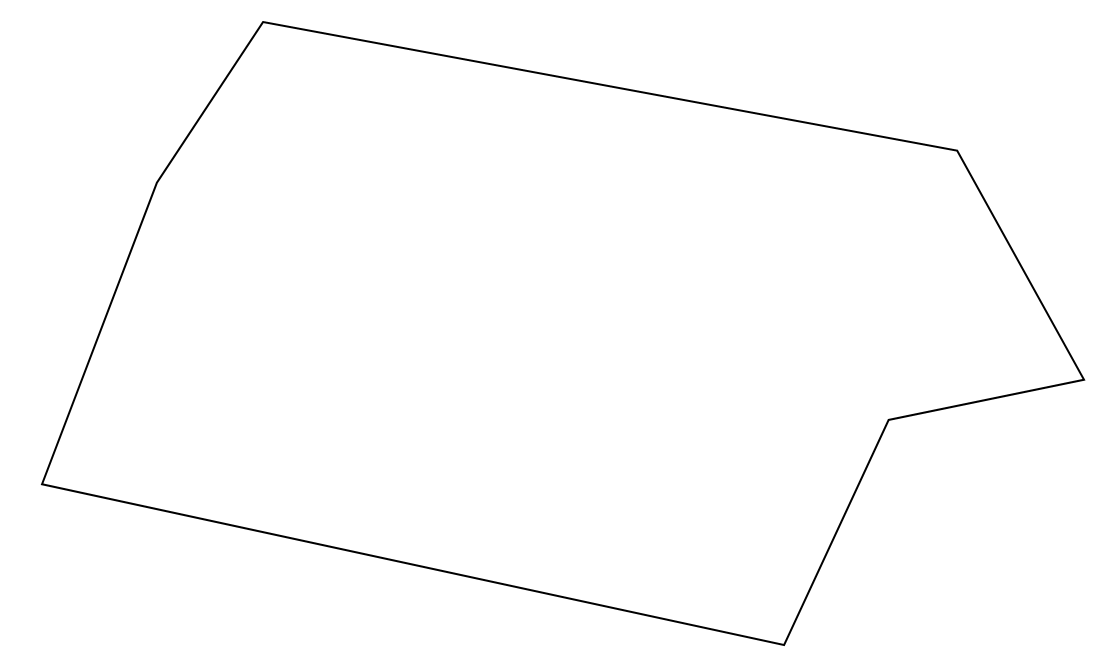
\includegraphics[width=68mm]{Chapters/MultiAgentCoverage/Figs/Polygon.PNG}\label{fig:PolygonOnly}
}
\subfloat[Bounding Rectangle Found]{
  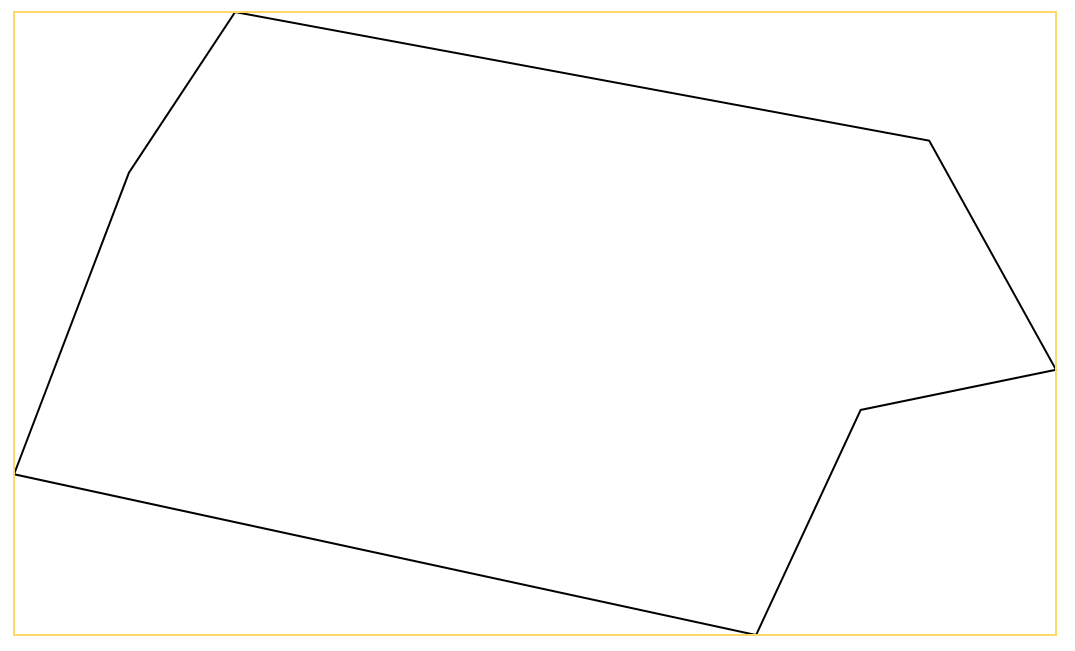
\includegraphics[width=68mm]{Chapters/MultiAgentCoverage/Figs/PolygonBoundingRect.PNG}\label{fig:PolygonWithBoundingRect}
}
\hspace{0mm}
\subfloat[Grid Points Generated in Bounding Rectangle]{
  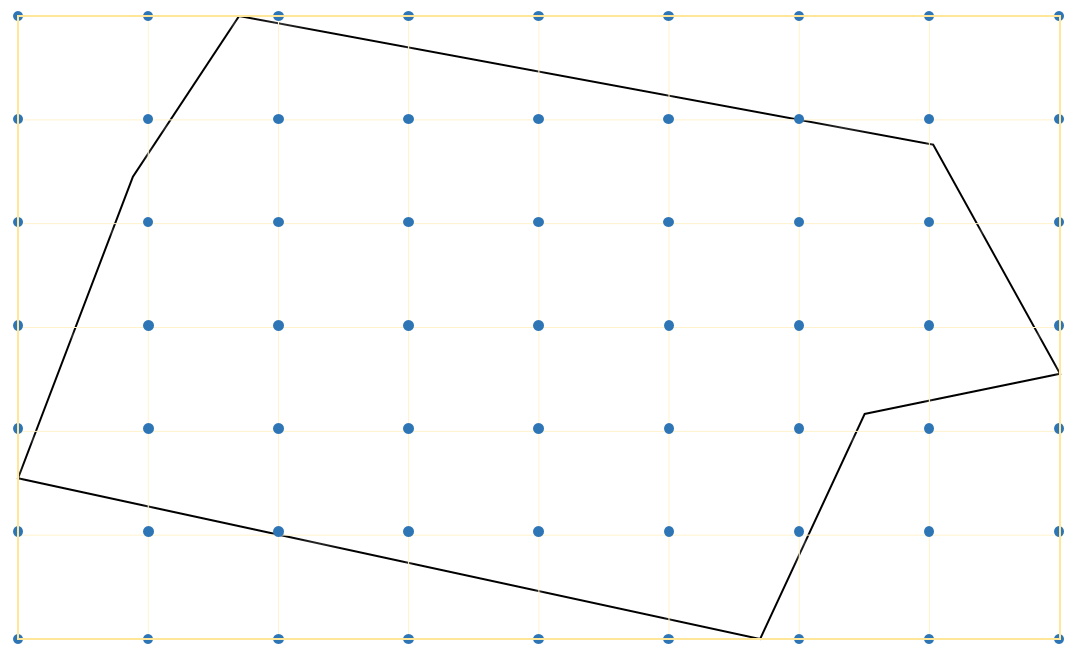
\includegraphics[width=68mm]{Chapters/MultiAgentCoverage/Figs/PolygonBoundingRectGridPoints.PNG}\label{fig:PolygonWithBoundingRectAndGridPoints}
}
\subfloat[Grid Points Outside of Polygon Pruned]{
  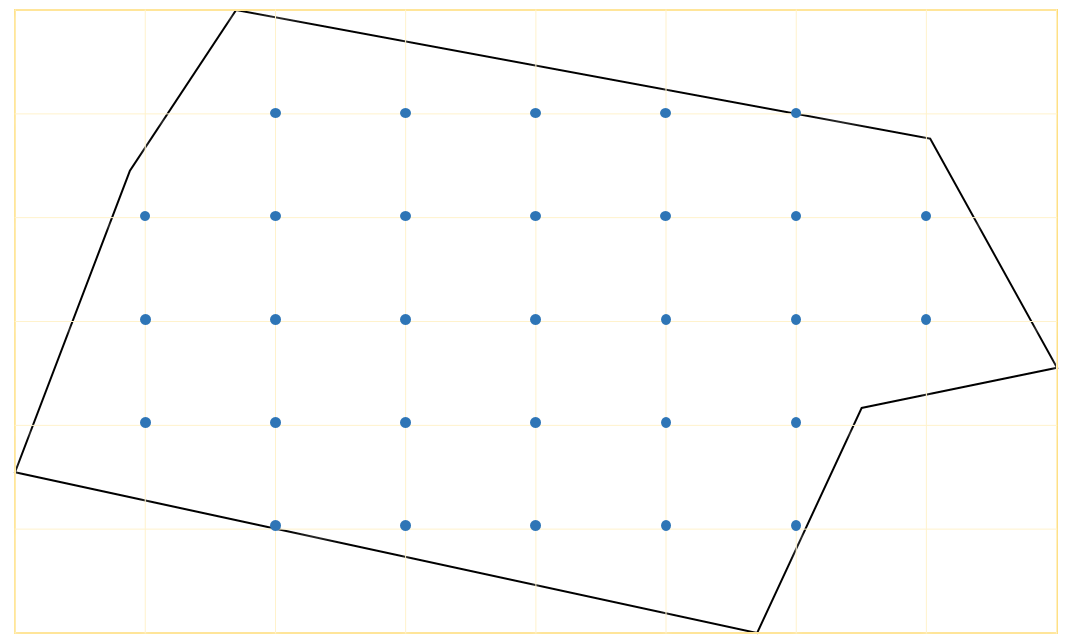
\includegraphics[width=68mm]{Chapters/MultiAgentCoverage/Figs/PolygonBoundingRectGridPointsPruned.PNG}\label{fig:PolygonWithBoundingRectAndGridPointsPruned}
}
\end{figure}

This procedure was devised with the aim of being straightforward to implement and modify. The algorithm used to carry out these steps is outlined in Algorithm \ref{alg:GridGeneration}. The algorithm is very intuitive: first, the bounding circum-rectangle is constructed from the largest and smallest x and y coordinates of the points in the polygon, outlined in lines 2-6. Then grid points in the bounding rectangle are generated in lines 7-13. Finally in lines 14-18, the grid points that lie inside the bounding rectangle but outside the polygon are pruned using the Point-in-Polygon routine which is described separately in Algorithm \ref{alg:PointInPolygon}. 


\begin{algorithm}{}
%\caption{Crossing Test for Point in Polygon based on \cite{Shimrat1962Algorithms}}
\caption{Point-in-Polygon}
\label{alg:PointInPolygon}
\begin{algorithmic}[1]
\renewcommand{\algorithmicrequire}{\textbf{Input:}}
\renewcommand{\algorithmicensure}{\textbf{Output:}}
%Input
\REQUIRE $ \newline R \quad \text{ The polygon which covers the region of interest}
%\newline R \quad \text{ The set of (x, y) points defining the polygon which covers the region of interest}
\newline P \quad \text{ A point which will be tested for containment in the polygon }
$
%Output
\ENSURE $\newline \text{True if P is contained in R else False }$

\hfill\pagebreak
\STATE polygon\_points $\leftarrow$ The set of points defining the vertices of R
\IF{x coordinate of $P$ is greater than the largest value or less than the smallest value of the x coordinates of the points in $R$}
\RETURN False
\ELSIF{y coordinate of $P$ is greater than the largest value or less than the smallest value of the y coordinates of the points in $R$}
\RETURN False


%\ELSIF{x coordinate of P is less than the smallest value of the x coordinate of all the points in R}
%\RETURN false
%\ELSIF{y coordinate of P is greater than the largest value of the y coordinate of all the points in R}
%\RETURN false
%\ELSIF{y coordinate of P is less than the smallest value of the y coordinate of all the points in R}
%\RETURN false

\ELSE
\STATE point\_in\_polygon $\leftarrow$ True
\STATE edges $\leftarrow$ the set of edges defining R
\FOR{each edge in edges}
\STATE p1 $\leftarrow$ the first point of edge
\STATE p2 $\leftarrow$ the second point of edge

\IF{(the y coordinate of $P$ lies between the  y coordinates of p1 and p2) \&
     the x coordinate of $P$ is less than the x coordinate of the point of intersection between e and the ray extended to +$\infty$ from $P$ in the +x direction}
\STATE point\_in\_polygon $\leftarrow \neg$ point\_in\_polygon
\ENDIF

\ENDFOR
\ENDIF
\end{algorithmic} 
\end{algorithm}


\begin{algorithm}{}
\caption{Algorithm to Generate a Uniformly Spaced Grid of Points in an Arbitrary Polygon}
\label{alg:GridGeneration}
\begin{algorithmic}[1]
\renewcommand{\algorithmicrequire}{\textbf{Input:}}
\renewcommand{\algorithmicensure}{\textbf{Output:}}
%Input
\REQUIRE $ \newline R \quad\text{ The set of (x, y) points defining the polygon which covers the region of interest}
\newline x\_spacing \quad\text{ The desired spacing between points in the x direction}
\newline y\_spacing \quad\text{ The desired spacing between points in the y direction}
$
%Output
\ENSURE $\newline grid\_points \quad \text{ A set of uniformly spaced (x, y) points, which define a regular } \newline \text{ tessellation of the region of interest}$

\hfill\pagebreak
\STATE grid\_points $\leftarrow$ empty array

\STATE max\_x $\leftarrow$ maximum x value of all points in R
\STATE min\_x $\leftarrow$ minimum x value of all points in R
\STATE max\_y $\leftarrow$ maximum y value of all points in R
\STATE min\_y $\leftarrow$ minimum y value of all points in R

\STATE bounding\_rect $\leftarrow$ The tightest bounding rectangle which contains the polygon R defined by the points (min\_x, min\_y), (min\_x, max\_y), (max\_x, max\_y),(max\_x, min\_y).

\STATE no\_y\_points $\leftarrow \left \lfloor{\frac{max\_y - min\_y}{y\_spacing}}\right \rfloor$
\STATE no\_x\_points $\leftarrow \left \lfloor{\frac{max\_x - min\_x}{x\_spacing}}\right \rfloor$

\FOR{y\_spacing\_index = 0 to no\_y\_points}
\FOR{x\_spacing\_index = 0 to no\_x\_points}
\STATE Add the point (min\_x + x\_spacing $\times$ x\_spacing\_index, min\_y + y\_spacing $\times$ y\_spacing\_index) to grid\_points
\ENDFOR
\ENDFOR
\FOR{point in grid\_points}
\IF{Point-in-Polygon(R, point) is false}
\STATE Remove point from grid\_points
\ENDIF
\ENDFOR
\RETURN grid\_points
\end{algorithmic} 
\end{algorithm}

%\begin{wrapfigure}{r}{0.5\textwidth}
%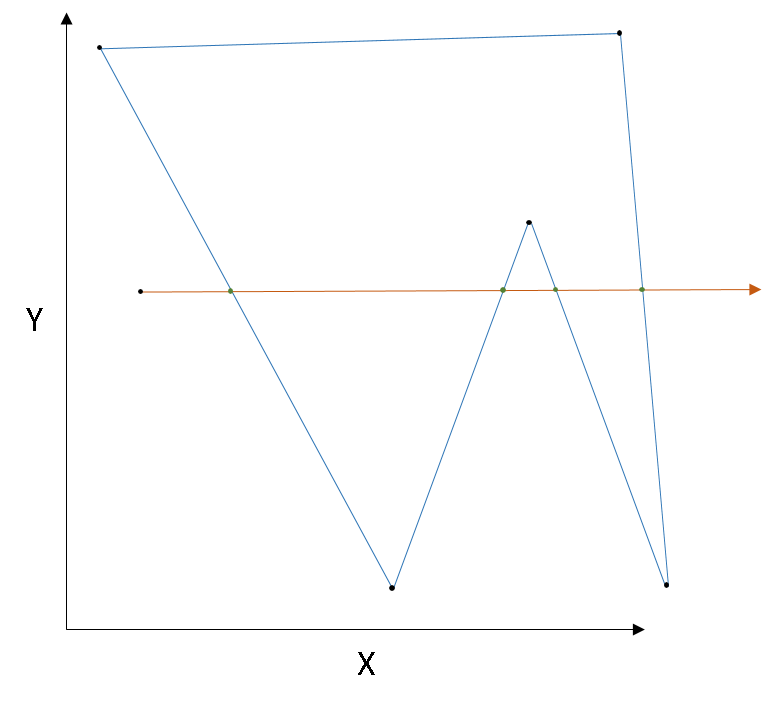
\includegraphics[width=65mm]{Chapters/MultiAgentCoverage/Figs/PointOutsidePolygon.PNG}\caption{Ray extended from point outside polygon intersects an even number of times}\label{fig:PointOutsidePolygon}
%\end{wrapfigure}

%\begin{wrapfigure}{r}{0.5\textwidth}
%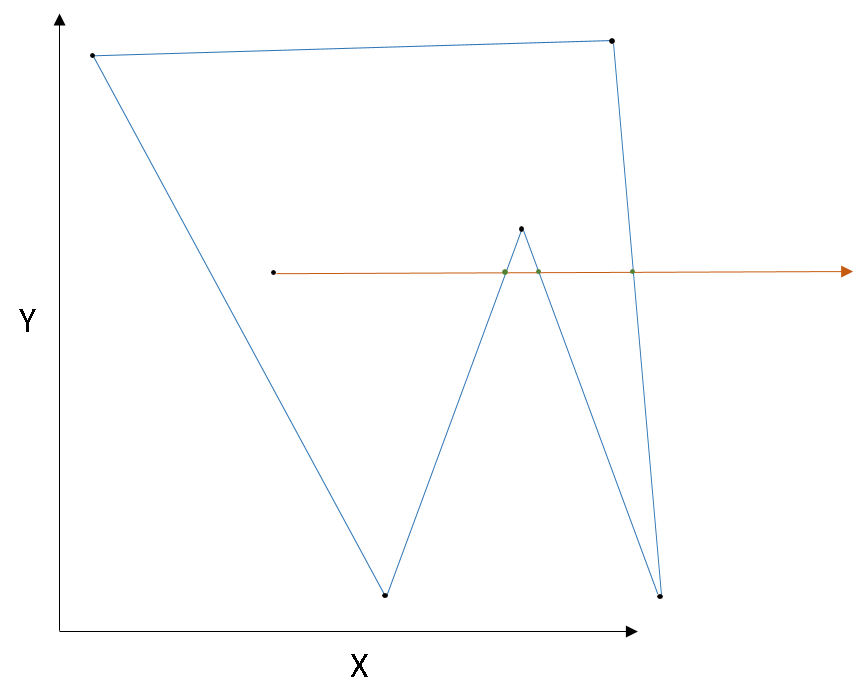
\includegraphics[width=65mm]{Chapters/MultiAgentCoverage/Figs/PointInsidePolygon.PNG}\caption{Ray extended from point inside polygon intersects an odd number of times}\label{fig:PointInsidePolygon}
%\end{wrapfigure}

We chose to use the well-known \textit{crossing test} \cite{Shimrat1962Algorithms}, which extends a ray from the point to be tested in the positive x-direction. If it crosses the boundary of the polygon an odd number of times, then it must be contained within it, otherwise it must lie outside it. This is illustrated in figures \ref{fig:PointOutsidePolygon} and \ref{fig:PointInsidePolygon}. The running time of this algorithm is dictated by the number of edges the polygon has and the size of the polygon relative to the desired tessellation spacing in the x and y directions. We did not make any optimizations other than the one outlined in lines 2-5 of Algorithm \ref{alg:PointInPolygon}, which checks whether the test point lies outside the largest and smallest x and y coordinates. but there is room to improve the running time significantly. This would be important if one is dealing with particularly large regions of interest or a relatively small spacing between grid points.


\begin{figure}{}
\subfloat[Ray extended from point outside polygon intersects an even number of times]{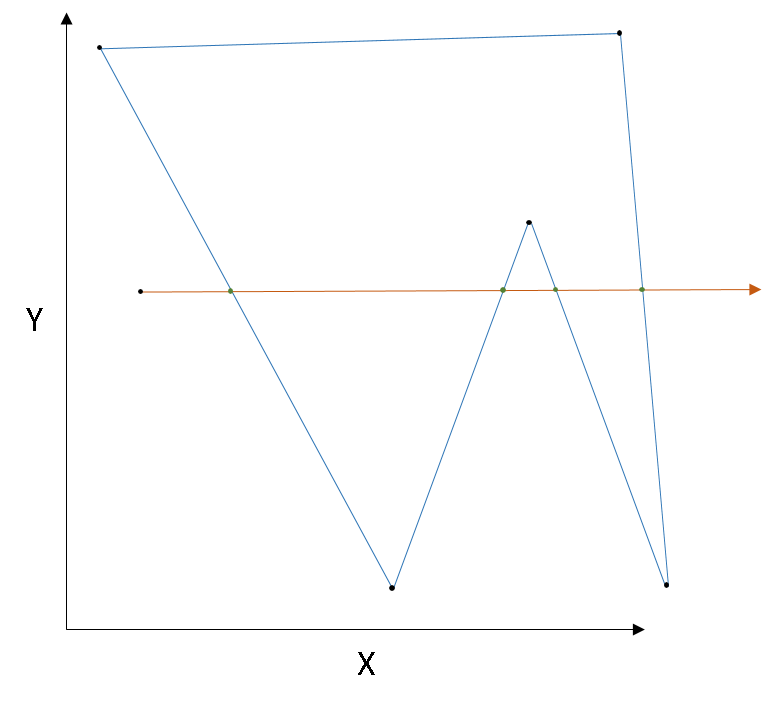
\includegraphics[width=60mm]{Chapters/MultiAgentCoverage/Figs/PointOutsidePolygon.PNG}\label{fig:PointOutsidePolygon}}
%\end{wrapfigure}
\hspace{1em}
\subfloat[Ray extended from point inside polygon intersects an odd number of times]{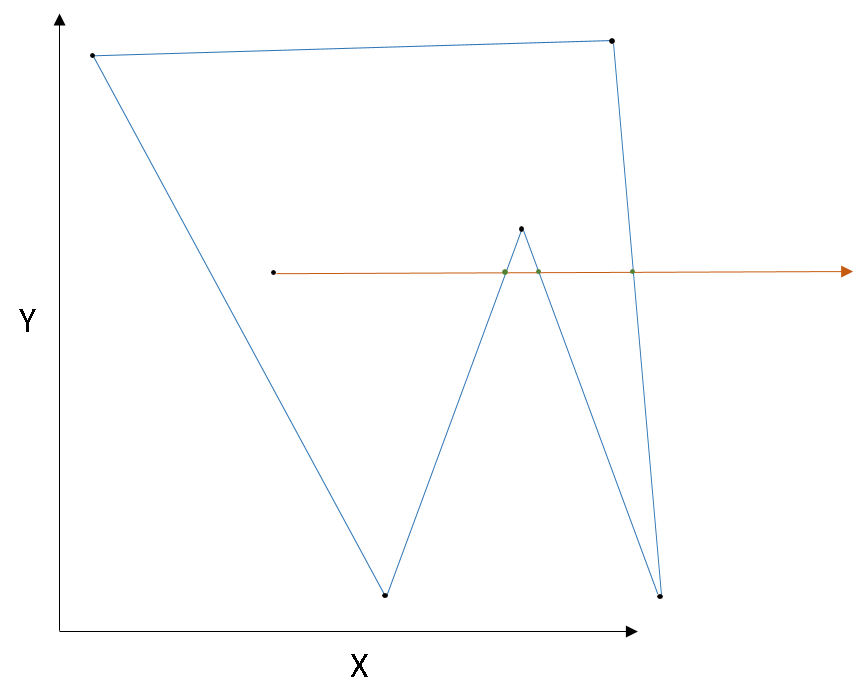
\includegraphics[width=60mm]{Chapters/MultiAgentCoverage/Figs/PointInsidePolygon.PNG}\label{fig:PointInsidePolygon}}
\end{figure}


%From a practical perspective, the region specified is defined over the earth's surface, which is not planar. For small regions, it can be assumed that this region is planar, since at 

%The generation of grid points takes this into account. The earth can be well described mathematically as an ellipsoid talk about WGS84



\subsection{Generating Waypoints as GPS Locations}
For the sake of real-world usage, it is necessary to refer to these points using some kind of reference coordinate system that UAVs can use. We provide a brief overview of how we accomplished this, without delving too far into Geographic Coordinate Systems (GCS). Since the textit{Global Positioning System} (GPS) is by far the most common system that UAVs use for navigation, we chose to design an implementation based on the \textit{World Geodetic System 1984} (WGS84) coordinate system, which is the coordinate system that GPS relies upon. The WGS84 system was created by the US department of defence and is officially documented in the official government report entitled "Department of Defense World Geodetic System 1984 Its Definition and Relationships With Local Geodetic Systems". It assumes that the datum surface is an oblate spheroid.
%, and the coordinate system uses Greenwich as the starting point. 
Coordinates are referenced using latitude, longitude and altitude, where longitude measurements range between [-180$^{\circ}$, 180$^{\circ}$], latitude measurements range between [-90$^{\circ}$, 90$^{\circ}$] and altitude measurements come in the form of meters above sea level. Greenwich is used as the \textit{prime meridian} for longitude, meaning Greenwich defines 0$^{\circ}$ longitude. The equator is used to define 0$^{\circ}$ latitude. In order to generate a grid of points in a bounding polygon as coordinates that can be referenced by the UAVs' GPS sensors, we had to make some modifications to the grid point generation algorithm outlined above. The main issue that arises is that the grid point generation algorithm assumes that the Cartesian coordinate system is used, which is obviously not valid when assuming coordinates lie on a  non-planar surface (the earth). We could simply treat the WGS84 coordinates that make the bounding polygon defining the region of interest as a plane and continue using the unmodified Algorithm \ref{alg:GridGeneration}, but for the sake of guaranteed accuracy we decided to make the following minor changes to the algorithm for use with WGS84 coordinates:
\begin{enumerate}
    \item When calculating distances, the well-known \textit{inverse solution} to finding geodesics (shortest paths along the earth's surface) is used. We also use the \textit{direct solution} to find a destination given a start point, bearing and distance. These algorithms are due to \citeauthor{Vincenty1975DirectEquations} and they take into account the non-planar nature of the WGS84 coordinate system \cite{Vincenty1975DirectEquations}. The inverse solution can be used in place of subtraction of Cartesian Coordinates and appears in lines 7 and 8 of Algorithm \ref{alg:GridGeneration} and line 12 of Algorithm \ref{alg:PointInPolygon}. The direct solution can be used in place of addition of distance to Cartesian coordinates and is used in line 11 of Algorithm \ref{alg:GridGeneration}.
    
    \item We created a specific WGS84 coordinate class, which can be used in place of regular Cartesian coordinates in Algorithms \ref{alg:GridGeneration} and \ref{alg:PointInPolygon}. We uploaded this to a publicly available  \href{https://github.com/DavidLSmyth/WGS84Coordinate}{github repository}\footnote{\href {https://github.com/DavidLSmyth/WGS84Coordinate}{https://github.com/DavidLSmyth/WGS84Coordinate}} with an MIT licence. If the user is not interested in generating grids which have very accurately spaced points, they can use the Cartesian solution which approximates the region of interest as a plane, otherwise the solution using Vincenty's equations in the point above can be applied.
\end{enumerate}

The code which allows the user to generate grids is hosted on github at <> \note{might be worth referencing how to pull it down using maven}

\subsection{User Interface and Results of Grid Generation Algorithm}
%to Facilitate Grid Generation
\note{Might not be worth talking about this in a full subsection}
We developed a User Interface (UI) in order to have the ability to quickly generate grids for use in simulations, as outlined in sections <target detection section> and <coverage section>. We also used the UI to visually validate that the grid generation code was performing as expected. We chose to use the  \href{https://shiny.rstudio.com/}{Shiny framework}\footnote{\href {https://shiny.rstudio.com/}{https://shiny.rstudio.com/}}, which is a web app development framework written in the \href{https://www.r-project.org/}{R language}\footnote{\href {https://www.r-project.org/}{https://www.r-project.org/}}. The Shiny framework is highly suited to prototyping web apps and abstracts away much of the more nuanced aspects of web development, at the cost of flexibility. We used the \href{https://rstudio.github.io/leaflet/}{Leaflet Package}\footnote{\href {https://rstudio.github.io/leaflet/}{https://rstudio.github.io/leaflet/}}, which provides a high-level interface to the \href{https://wiki.openstreetmap.org/wiki/Develop}{Open Street Map}\footnote{\href {https://wiki.openstreetmap.org/wiki/Develop}{https://wiki.openstreetmap.org/wiki/Develop}} API. We added an \textit{observeEvent} function to record when the user clicks on points on the map, adding an edge the previously clicked point to the current clicked point. The process of sequentially selecting the points on the map defining a polygonal region can be seen in figure \ref{fig:AddClicks}. 

\begin{figure}{}
\subfloat{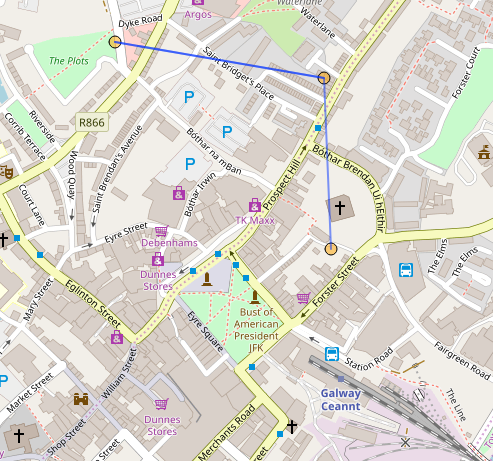
\includegraphics[width=48mm]{Chapters/MultiAgentCoverage/Figs/AdditionalClicks.PNG}}
%\end{wrapfigure}
\hspace{0.2em}
\subfloat{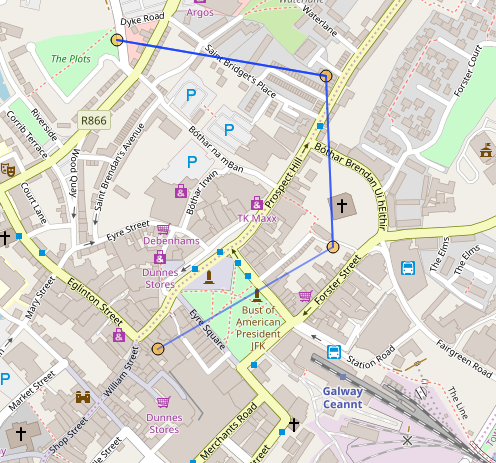
\includegraphics[width=48mm]{Chapters/MultiAgentCoverage/Figs/AdditionalClicksOne.PNG}}
\hspace{0.2em}
\subfloat{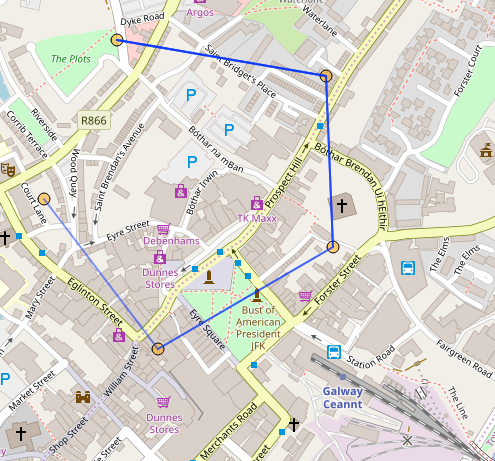
\includegraphics[width=48mm]{Chapters/MultiAgentCoverage/Figs/AdditionalClicksTwo.PNG}}
\caption{Creating the bounding polygon using the UI}
\label{fig:AddClicks}
\end{figure}

In order to actually generate and draw the grid points on the user interface, we added "Show planned waypoints" button. When this button is clicked, the polygon defining the region of interest that the user has selected is sent to the grid generation code, as well as the desired latitude and longitude spacing between the generated grid points. The grid points are generated and written to a file. The user interface then reads this points from the file and then overlays them on the map. Examples of visualisation of polygonal regions with grid points are shown in figure \ref{fig:GridPointsOnUI}. This code has been open-sourced with an MIT licence and and be found on 
\href{https://github.com/NUIG-ROCSAFE/CBRNeVirtualEnvironment}{ Github.}\footnote{\href {https://github.com/NUIG-ROCSAFE/CBRNeVirtualEnvironment}{https://github.com/NUIG-ROCSAFE/CBRNeVirtualEnvironment}}

\begin{figure}{}
\centering
\subfloat[Grid points with a latitude spacing of 40m and a longitude spacing of 30m.]{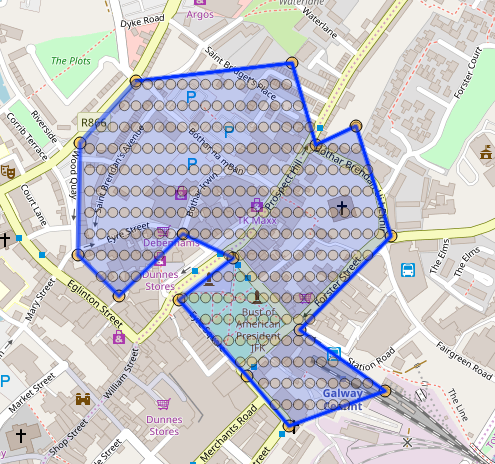
\includegraphics[width=70mm, height=65mm]{Chapters/MultiAgentCoverage/Figs/RegionOne.PNG}}
%\end{wrapfigure}
\hspace{0.2em}
\subfloat[Grid points with a latitude spacing of 30m and a longitude spacing of 25m.]{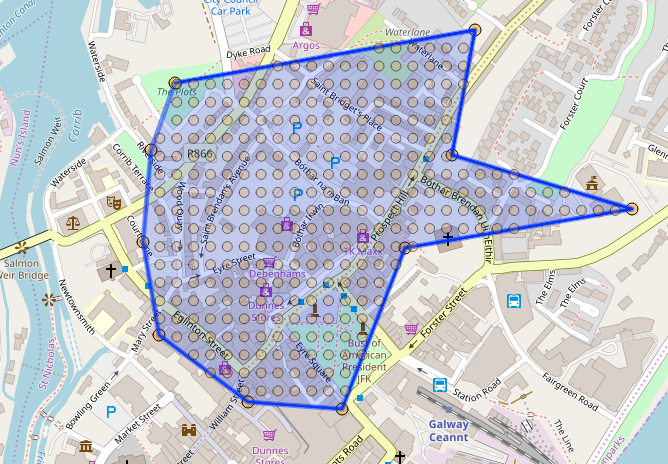
\includegraphics[width=70mm, height=65mm]{Chapters/MultiAgentCoverage/Figs/RegionTwo.PNG}}
\caption{Examples of generated grid points overlaid onto the UI}
\label{fig:GridPointsOnUI}
\end{figure}


\note{Make sure to refer to target localisation}

















%\nomenclature[]{VRP}{Vehicle Routing Problem}

\section{Scene Surveying}\label{sec:SceneSurveying}
This section outlines the algorithms that were explored to generate a set of routes for the RAVs that will be used to record sensor data at each of the grid points generated in the region of interest. We gave a high-level description of this problem at the beginning of Chapter \ref{chapter:SceneSurveying}:
"\textit{Find a set of routes for each of $K$ RAVs to be used in the data-gathering process, such that these sets partition $R$ and the cost of the system of RAVs traversing these points is minimized}".
%which are generated using Algorithm \ref{alg:GridGeneration} described in the preceding section. 
We make some assumptions related to the solution of this problem:
\note{This list might not cover everything, come back to it}
\begin{itemize}
    \item Each RAV is assumed to have the same internal representation of the region of interest, namely the set of uniformly spaced grid points generated by Algorithm \ref{alg:GridGeneration}.
    \item Each RAV is assumed to have the ability to move between any pair of grid points unobstructed using the shortest possible path.
    \item RAVs are assumed to move with a fixed operational velocity, which can vary between RAVs.
    \item Each RAV may be equipped with different sensors to the others and it is assumed that sensing times may vary among the RAVs.
    \item Each RAV has a finite battery capacity which implies they have a finite amount of time that they can fly for before they need to recharge.
\end{itemize}

%Talk about how problem was transformed to TSP problem, took that and then divided up soln for mTSP.

The scene surveying problem that we would like to solve can be treated as an instance of the \textit{Vehicle Routing Problem} (VRP), which was first described in a paper by \citeauthor{Dantzig1959TheProblem} \cite{Dantzig1959TheProblem}. This problem is a generalisation of the classic \textit{Travelling Salesman problem} (TSP). There are many variants and extensions to this problem, but the VRP essentially asks for a set of routes to be assigned to the RAVs such that each point in the graph is visited exactly once, which minimises the total time taken to "service" each of the points \cite{Dantzig1959TheProblem}. In our case, the service time is the time taken to record a sensor reading. We are interested in solving this problem where the graph is defined by the grid of points that is generated using Algorithm \ref{alg:GridGeneration}. A formal definition of the VRP and its variants can be found in \cite{Toth2002TheProblem}.

\subsection{Simplified Problem}\label{subsec:SimplifiedVRP}
\note{maybe change this to constrained problem or something similar}
We began by taking a simplified version of the full vehicle routing problem in order to explore possible solutions. This section expands on our published work in \cite{Smyth2018UsingDrones}, which summarises how this simplified problem was tackled. Rather than concern ourselves with the details of sensor sampling times and battery constraints, we first focused on designing a solution that can assign a set of routes to a homogeneous set of RAVs. 
%We assumed that service times add a fixed constant to the total time taken to perform the survey (and can hence be ignored) and we ignore the time added that the RAVs might need to recharge. 
The problem can be described as follows:
\\
\textit{Given a fully connected graph, $G$, to visit and $n$ RAV agents, find a subtour for each agent such that each point in $P \in G$ is visited exactly once by any agent in the system, with the objective of minimizing the longest time taken for any individual agent subtour, in order to minimize the time taken to carry out the survey.}
\\
This is the \textit{multiple Travelling Salesman Problem} (mTSP). 

%According to the number of distribution centers: single distribution center and multi-distribution center problem;
%According to the type of vehicle: single-vehicle type and multi-vehicle type problem;
%According to the characteristics of the task: pure send (take) cargo problems and loading and unloading mixing problem;
%According to whether the time constraints: no time window problem and time window problem;
%By vehicle loading: And the problem of non-full load;
%According to the optimization of the number of goals: a single objective and multi-objective problem;
%Vehicle and vehicle by the ownership of the points: the vehicle open problem and vehicle closure problems;
%By mastering the information of certainty: Sexual VRP and non-deterministic VRP problems;
%As can be seen from these classifications, solutions to the VRP problem are varied, each category 

\subsection{Proposed Solution for the Simplified Problem}
\note{Again maybe use constrained instead of simplified}
Due to the fact that the mTSP is at least as hard as the TSP, since it is a generalisation of the TSP, finding a polynomial time solution to the mTSP is not feasible. We explored a number of sub-optimal solutions that take advantage of the highly structured nature of the uniformly spaced grid that we use in our instance of the problem. The usual trade-off between solution quality vs. time taken to find the solution motivated our choice of implemented algorithm, as we anticipated that the time taken to execute the planned routes may be comparable to the time taken to generate some solutions (the order of minutes or hours). For example, \citeauthor{Hungerlander2018TheGrids} shows the results of using a Mixed Integer Linear Program (MILP) took hours to run for grid sizes that could be considered relatively small in many real-world domains \cite{Hungerlander2018TheGrids}.
%which would exceed the amount of time taken to perform even a random solution. %General details of solutions that can be applied to solve the mTSP and VRP can be found in Section <> of the literature review (this will be filled in).

\subsection{Nearest Neighbor Algorithm}
There are four common heuristic algorithms that form the basis of most solutions to TSP and mTSP problems, as stated in \cite{Johnson1997TheOptimization}: the \textit{nearest neighbor} algorithm, the \textit{greedy algorithm}, the \textit{Clarke-Wright} algorithm and the \textit{Christofides} algorithm. We began by implementing an algorithm which is a modification of a TSP solution based on the nearest-neighbor heuristic. Our reasoning is based on the following premises:
\begin{enumerate}
    \item The nearest-neighbor heuristic is a well-known heuristic that is straightforward to implement. It is known to provide good results to the TSP when the cost is defined as the Euclidean distance between points \cite{Johnson1997TheOptimization}, as in our use case.
    \item The nearest-neighbor solution to the TSP can be very easily modified to be applied to the mTSP by implementing it in a round-robin manner, as detailed in Algorithm \ref{alg:NNHeuristic}.
    \item The nearest-neighbor heuristic is known to have a running time which is O($n^2$) \cite{Rosenkrantz1977AnProblem}, which means it can scale well to reasonably large problem instances compared to other algorithms which have a far worse performance complexity. For example, the Christofides algorithm is known to be within a factor of $\frac{3}{2}$ of the optimal solution, but its running time is O($n^3$) \cite{Christofides1976WORST-CASEPROBLEM}, which quickly becomes prohibitively long.
    %\item Partitioning a TSP solution can give very good mTSP solutions on the same graph.
\end{enumerate}

The nearest-neighbor (NN) heuristic algorithm for the multiple Travelling Salesman problem is shown in Algorithm \ref{alg:NNHeuristic}.


\begin{algorithm}[h]
\caption{The Nearest-Neighbor Solution to the mTSP Problem}
\label{alg:NNHeuristic}
\begin{algorithmic}[1]
\renewcommand{\algorithmicrequire}{\textbf{Input:}}
\renewcommand{\algorithmicensure}{\textbf{Output:}}

\REQUIRE$ \newline k: \quad \text{ The number of RAVs in the mTSP }
\newline way\_points: \quad \text{ The set of points the RAVs must visit }
\newline cost(i,j): \quad \text{ The function giving the cost of travelling from node i to node j }
$
\ENSURE $ \newline RAV\_routes: \quad \text{A key-value data structure mapping RAVs to their corresponding routes.}
$

\hfill\pagebreak

%\noindent\textbf{\textit{\noindent Initialization} :}\\
\STATE RAV\_routes$\leftarrow$empty key-value container
\STATE visited\_points$\leftarrow$empty array
\STATE remaining\_points\_to\_visit$\leftarrow$way\_points
\FOR{each agent in agents:}
%\quad 
\STATE Initialise path of agent as empty array in RAV\_routes
\ENDFOR

current\_agent\_index$\leftarrow$0\\
%current\_agent$\leftarrow$agents.get(current\_agent\_index)\\
\hfill\pagebreak
\WHILE {pointsToVisit is not empty}
\STATE agent\_position $\leftarrow$ last value in agent\_paths.get(current\_agent\_index)
\STATE nearest\_neighbor$\leftarrow$\(\displaystyle \min_{neighbor \in points\_to\_visit}\)cost(agent\_position, neighbor)
\STATE Update current\_agent value in agent\_paths to include nearest\_neighbor
\STATE Add nearest\_neighbor to visited\_points.
\STATE Remove nearest\_neighbor from remaining\_points\_to\_visit.
\STATE current\_agent\_index$\leftarrow$(currentAgentIndex+1) $\mathbf{mod}$$\vert$List of Agents$\vert$

%\STATE currentAgent$\leftarrow$agents.get(currentAgentIndex)


\ENDWHILE
\RETURN RAV\_routes
\end{algorithmic} 
\end{algorithm}

\begin{figure}[h]
\centering
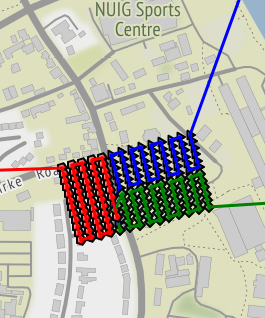
\includegraphics[width=0.5\textwidth]{Chapters/MultiAgentCoverage/Figs/RAVRoutingNUIGCropped.png}
\caption{NN heuristic encourages the creation of optimal sub-tours, which are assigned to each RAV}
\label{fig:NNPartitioning}
\end{figure}

The algorithm can be seen to be a very straightforward extension of the single agent NN algorithm. The while loop iteratively cycles through the list of RAVs and assigns the nearest non-assigned neighbor to the next RAVs partially assembled route.

Since we run this algorithm over a uniformly-spaced grid, it builds agent routes in a lawn-cutting pattern, which provides good results as long as the routes do not begin to overlap. The idea is to take the NN algorithm TSP solution and apply it exhaustively in a round-robin manner, so that each RAV is encouraged to find a non-overlapping optimal sub-tour. These non-overlapping optimal sub-tours partition the region and therefore offer a solution to the mTSP. Section 4 of \cite{Hungerlander2018TheGrids} gives an insight to how optimal solutions can be found for a uniformly spaced rectangular grid when RAVs are assumed to start in the corners of the rectangle, which provides further motivation to using Algorithm \ref{alg:NNHeuristic}. In practice non-overlapping optimal sub-tours are not found, but solutions may come close, as illustrated in Figure \ref{fig:NNPartitioning}.

%Since sometimes the solutions found by the algorithm are not always well-balanced, we propose to iteratively re-run the algorithm after a set interval in order to update the solution to ensure that no RAV is idle while others are doing work. This also ensures redundancy in the system - if a RAV stops operating, its uncompleted work will be re-assigned to the others.

%\note{Not sure if worth mentioning lower bound of cost for this algo is 1/noRAVs}
%\note{might be worth mentioning that it would be ideal to add the next grid point to whichever agent has the shortest route so far}



\subsection{Analysis of the NN algorithm}
%\note{The justification behind this choice of algo is a bit weak, might be worth running tests on file:///C:/Users/13383861/Downloads/graphsOR18.pdf}


The results and analysis of applying the NN heuristic algorithm to the symmetric Euclidean TSP and mTSP are well documented and we will not go into great detail repeating the results here. Instead, we refer the reader to the chapter ``The travelling salesman problem: A case study'' of \cite{Aarts:1997:LSC:549160}, written by \citeauthor{Johnson1997TheOptimization}, which provides a comparison of the NN heuristic to other heuristic algorithms. They compare solutions with the standard Held-Karp lower bound \cite{Held1962AProblems} using a standardised library of Travelling Salesman Problems, TSPLIB \cite{TSPLIB}. Rather than provide tables of results showing the performance of the NN heuristic algorithm on standard benchmark data sets such as TSPLIB, we instead focus on the results for the domain we are most interested in, which is a connected graph defined by a uniformly spaced set of grid points. We found that the algorithm performed best when the RAVs used regions that have multiple axes of symmetry. Rectangular regions in particular yield scalable, high-quality solutions, as shown in the figures in Table \ref{table:NNAlgoResultsRect}. This corresponds to the optimal performance configuration suggested in \cite{Hungerlander2018TheGrids}. We evaluated solutions both qualitatively and  quantitatively. We focused on the qualitative results of the experiments, which were designed to show that the system can partition the in the region to give a reasonably balanced amount of work to each agent for regular polygons with a number of axes of symmetry. This was a proof-of-concept, with the intention for future work to provide a more thorough analysis on performance. We found that RAV starting points are a critical factor in solution quality, which again is in line with the findings in \cite{Hungerlander2018TheGrids}. Tables \ref{table:NNAlgoResultsRect}, \ref{table:NNAlgoResultsTri} and \ref{table:NNAlgoResultsHex} %\ref{table:NNAlgoResultsIrregular} 
illustrate some of the results, with the configuration of each listed below. The experiments are intended to demonstrate practical use cases where the NN algorithm will provide qualitatively good results.

\pagebreak
\subsection{Qualitative Behaviour of the NN Algorithm With a Rectangular Grid}
We set up this experiment with the aim of showing that if the RAVs can be placed in the configuration suggested by \citeauthor{Hungerlander2018TheGrids}, they will partition the region in a close to optimal fashion \cite{Hungerlander2018TheGrids}, minimising the longest distance any one RAV needs to travel to complete its mission. We ran the experiment using 1-4 RAVs, placing them in the corners of the rectangles. This was done in an approximate fashion by manually dragging the RAVs to their starting position using the UI mentioned in Section \ref{subsec:SceneSurveyingUI}. The results in Table \ref{table:NNAlgoResultsRect} show that the amount of work done by each RAV is approximately evenly balanced. Theoretically, the minimum amount of work done by each RAV would be $\frac{1}{2}$, $\frac{1}{3}$ and $\frac{1}{4}$ of the total work done by a single RAV when using 2, 3 and 4 RAVs respectively.
\par The results show that when using 2, 3 and 4 RAVs, the solutions found by the NN algorithm were 2.701\%, 4.500\% and 17.315\% less efficient than evenly splitting up the solution for a single RAV ( $\frac{1}{2}$, $\frac{1}{3}$ and $\frac{1}{4}$ of 3576.6m of the single-RAV route length, respectively). This was partly due to the extra distance added from the starting positions. Note that when using 4 RAVs, there was some overlap in the routes which added a significantly higher overhead to the cost of the route in relation to that given by even splitting the solution found for a single RAV.


We used the following configuration to run the experiment:
\\Spacing between grid points: 23m in latitude, 25m in longitude.
\\Bounding rectangle coordinates: (53.2781933786, -9.0671226391), (53.2803800539, -9.067182416), (53.2804392784, -9.0611222377), (53.2782526061, -9.0610624609)
\\

\begin{table}[H]
  \centering
  \begin{tabular}{ | c | m{5cm} | }
    \hline
    Planned RAV Routes & Route Lengths (metres) \\
    \hline
    
    %single RAV
    \begin{minipage}[c][53mm][c]{.6\textwidth}
      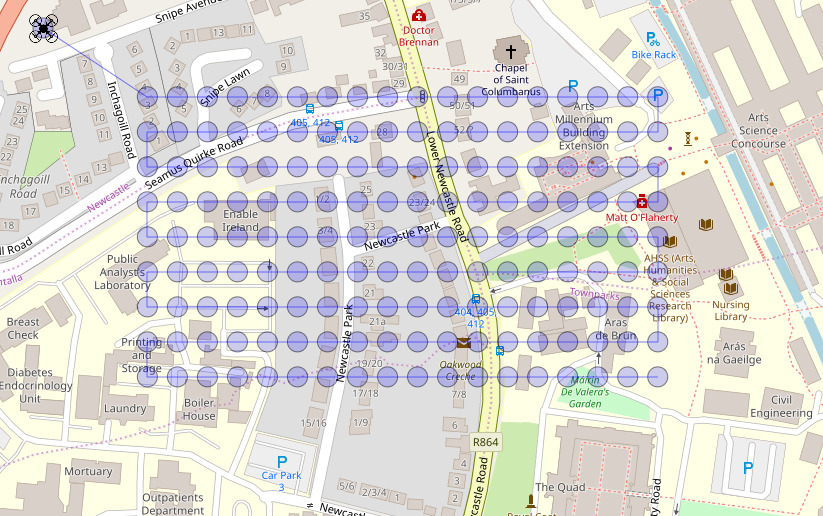
\includegraphics[width=\linewidth, height=51mm]{Chapters/MultiAgentCoverage/MultipleTravellingSalesman/Figs/Rectangle/SingleAgent.PNG}

    \end{minipage}
    &
    \begin{itemize}[leftmargin=*]
      \item[] RAV 1 (blue): 3576.6
    \end{itemize}
    \\
    \hline
    %two RAV
    \begin{minipage}[c][53mm][c]{.6\textwidth}
      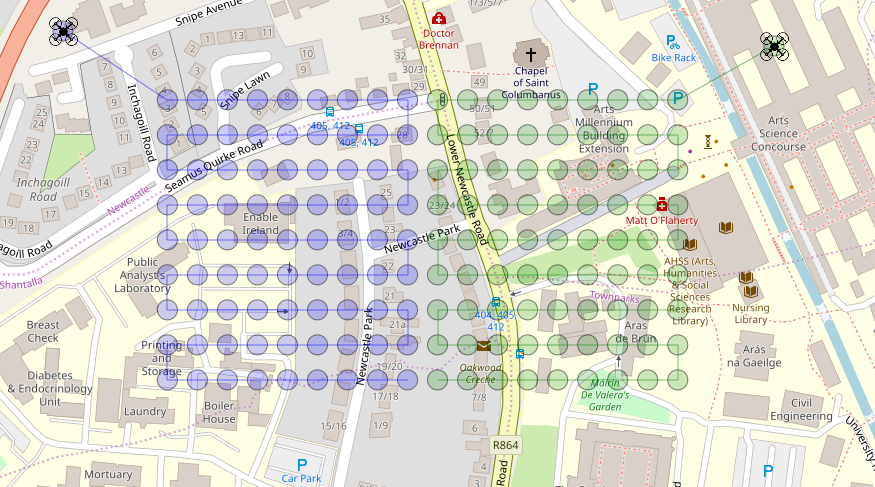
\includegraphics[width=\linewidth, height=51mm]{Chapters/MultiAgentCoverage/MultipleTravellingSalesman/Figs/Rectangle/TwoAgent.PNG}
    \end{minipage}
    &
    \begin{itemize}[leftmargin=*]
        \item[] RAV 1 (blue): 1836.3
        \item[] RAV 2 (green): 1825.8
    \end{itemize}
    \\
    \hline
    
    %three RAV
    \begin{minipage}[c][53mm][c]{.6\textwidth}
      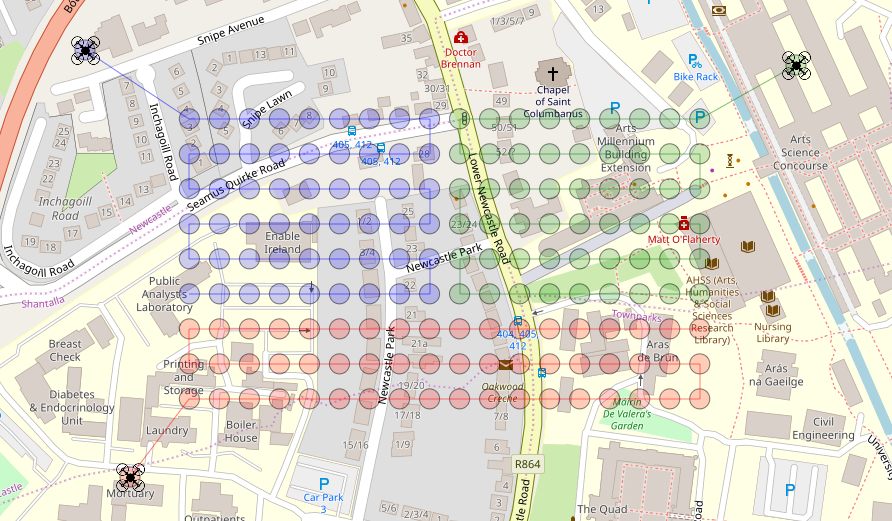
\includegraphics[width=\linewidth, height=51mm]{Chapters/MultiAgentCoverage/MultipleTravellingSalesman/Figs/Rectangle/ThreeAgent.PNG}
    \end{minipage}
    &
    \begin{itemize}[leftmargin=*]
    \item[] RAV 1 (blue): 1245.6
    \item[] RAV 2 (green): 1235.1
    \item[] RAV 3 (red): 1215.9
    \end{itemize}
    \\
    \hline
    
    %Four RAV
    \begin{minipage}[c][53mm][c]{.6\textwidth}
      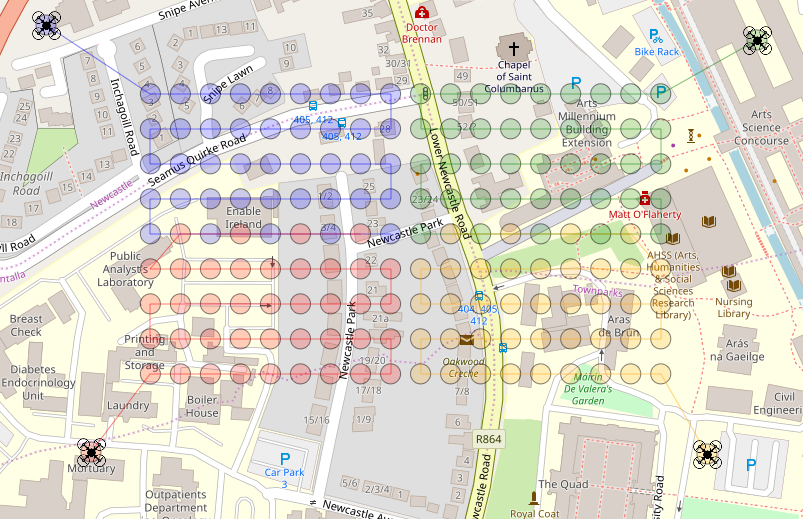
\includegraphics[width=\linewidth, height=51mm]{Chapters/MultiAgentCoverage/MultipleTravellingSalesman/Figs/Rectangle/FourAgent.PNG}
    \end{minipage}
    &
    \begin{itemize}[leftmargin=*]
    \item[] RAV 1 (blue): 1048.8
    \item[] RAV 2 (green): 1038.3
    \item[] RAV 3 (red): 994.5
    \item[] RAV 4 (yellow): 990.5
    \end{itemize}

    \\
    \hline
  \end{tabular}
  \caption{Results of applying NN algorithm to a rectangular region}\label{table:NNAlgoResultsRect}
\end{table}




\pagebreak
\subsection{Qualitative Behaviour of the NN Algorithm With a Triangular Grid}
This experiment was set up in a similar manner to the first, where the RAVs were dragged to an initial starting position that should allow the NN algorithm to take advantage of the axes of symmetry of the triangle.
The results in Table \ref{table:NNAlgoResultsTri} show that the amount of work done by each RAV is approximately evenly balanced when using two RAVs, but not three. 

The results show that when using two and three RAVs, the solutions found by the NN algorithm were 0.155\% and 36.565\% less efficient than that given by even splitting the solution for a single RAv ( $\frac{1}{2}$ and $\frac{1}{3}$ of 1940.6, respectively). This can be explained by the corresponding figures displaying the agents routes in Table \ref{table:NNAlgoResultsTri}. Clearly, the NN algorithm takes advantage of the symmetry down the vertical center axis when two RAVs are used, but when three RAVs are used, the solution the RAV beginning at the top of the triangle skips the grid points that require a "diagonal" move, instead moving down to the closer grid point. These points are picked up by the second RAV (green) once it meets the third (red), adding a relatively large cost.

We used the following configuration to run the experiment:
\\Spacing between grid points: 23m in latitude, 25m in longitude.
\\Bounding rectangle coordinates: (53.2781933786, -9.0671226391), (53.2782526061, -9.0610624609), (53.2803800539, -9.06409255)
\\

%\\Spacing between grid points: 23m in latitude, 25m in longitude.
%\\Bounding rectangle coordinates: (53.2781933786, -9.0671226391), (53.2782526061, -9.0610624609), (53.2803800539, -9.06409255)
\begin{table}[H]
  \centering
  \begin{tabular}{ | c | m{5cm} | }
    \hline
    Planned RAV Routes & Route Lengths (metres) \\
    \hline
    
    %single RAV
    \begin{minipage}[c][57mm][c]{.6\textwidth}
      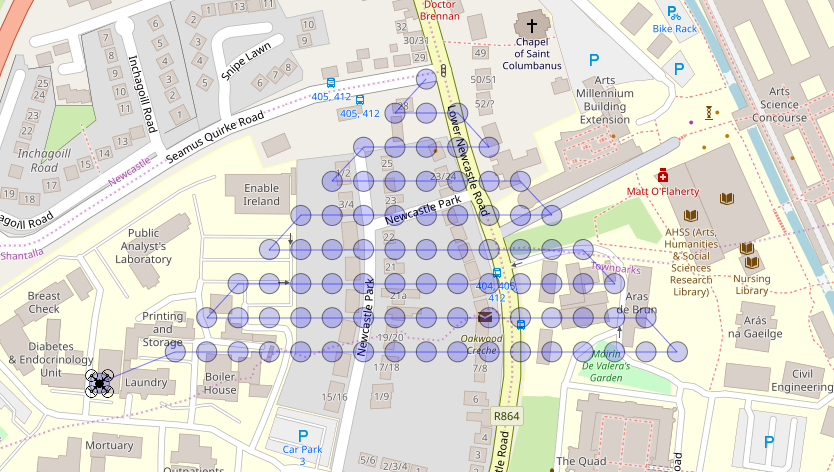
\includegraphics[width=\linewidth, height=55mm]{Chapters/MultiAgentCoverage/MultipleTravellingSalesman/Figs/Triangle/OneRAV.PNG}
    \end{minipage}
    &
    \begin{itemize}[leftmargin=*]
      \item[] RAV 1 (blue): 1940.6
    \end{itemize}
    \\
    \hline
    %two RAV
    \begin{minipage}[c][57mm][c]{.6\textwidth}
      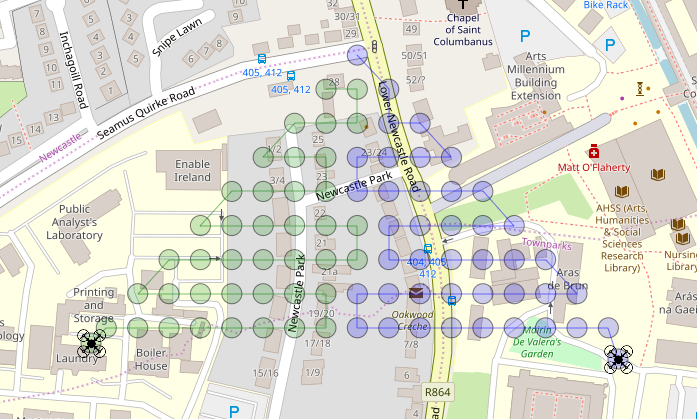
\includegraphics[width=\linewidth, height=55mm]{Chapters/MultiAgentCoverage/MultipleTravellingSalesman/Figs/Triangle/TwoRAV.PNG}
    \end{minipage}
    &
    \begin{itemize}[leftmargin=*]
        \item[] RAV 1 (blue): 971.8
        \item[] RAV 2 (green): 930.7
    \end{itemize}
    \\
    \hline
    
    %three RAV
    \begin{minipage}[c][57mm][c]{.6\textwidth}
      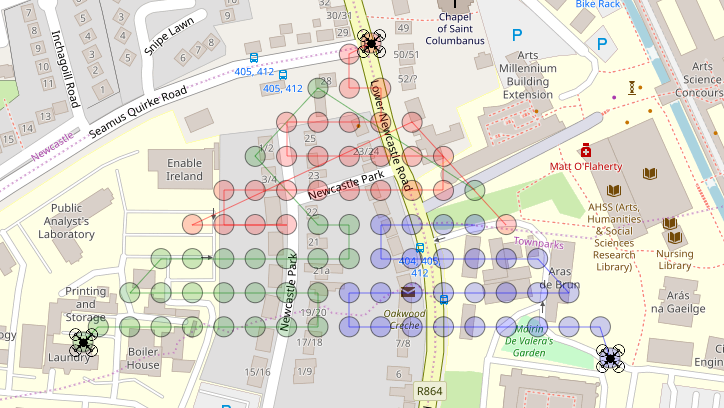
\includegraphics[width=\linewidth, height=55mm]{Chapters/MultiAgentCoverage/MultipleTravellingSalesman/Figs/Triangle/ThreeRAV.PNG}
    \end{minipage}
    &
    \begin{itemize}[leftmargin=*]
    \item[] RAV 1 (blue): 621.6
    \item[] RAV 2 (green): 812.7
    \item[] RAV 3 (red): 883.4
    \end{itemize}
    \\
    \hline
  \end{tabular}
  \caption{Results of applying NN algorithm to a triangular region}\label{table:NNAlgoResultsTri}
\end{table}


%\textbf{Hexagonal Region}
%\\Spacing between grid points: 32m in latitude, 38m in longitude.
%\\Bounding rectangle coordinates: (53.2782526061, -9.0610624609), (53.2803800539, -9.06409255), (53.2781933786, -9.0671226391), (53.27621, -9.0671226391), (53.27402, -9.06409255), (53.27615, -9.0610624609)
%\\



\pagebreak
\subsection{Qualitative Behaviour of the NN Algorithm With a Hexagonal Grid}
This experiment was again set up in a similar manner to the first, where the RAVs were dragged to starting positions that should allow the NN algorithm to take advantage of the axes of symmetry of the hexagon. In this case, we had to vary their starting locations depending on the number of RAVs used in order to encourage the generation of non-overlapping solutions. We found that the NN algorithm could find (approximately) symmetrical solutions using two or four RAVs, shown in Table \ref{table:NNAlgoResultsHex}.



The results show that when using two RAVs, the longest route is 2.191\% shorter than half the length of the route found using just one RAV. When two RAVs are used, they move horizontally to the nearest grid location, meet in the middle of the hexagon and then move back to the outer edge. Once the reach the lower third of the hexagon, they move down diagonally and then back across horizontally. This behaviour is the same when using a single RAV. The key difference is when they move to the top third of the hexagon, they exhibit the same behaviour, wheras the single agent skips some of the "diagonal" grid points, as in the case of the triangular region using three RAVs. It must go back to visit them at a relatively large cost, since the points that it missed on each from range from both the left and right sides of the upper hexagon. This can be seen in the first figure in Table \ref{table:NNAlgoResultsHex}.


When using four RAVs, the longest route was 36.565\% longer than $\frac{1}{4}$ of the length of the route found for a single RAV. This was mainly due to the slight imbalance in the number of points in the upper third and lower third of the hexagon and the middle third. There are 79 points in both the upper and lower third and 147 points in the middle third. This means that the two RAVs that sweep back and across the middle move to the upper and lower third to "help". This results in large jumps to finish of the final few grid points, visible in the third figure of Table \ref{table:NNAlgoResultsHex}. 

We used the following configuration to run the experiment:
\\
Spacing between grid points: 32m in latitude, 38m in longitude.
Bounding coordinates: (53.2782526061, -9.0610624609), (53.2803800539, -9.06409255), (53.2781933786, -9.0671226391), (53.27621, -9.0671226391), (53.27402, -9.06409255), (53.27615, -9.0610624609)





\begin{table}[H]
  \centering
  \begin{tabular}{ | c | m{4.5cm} | }
    \hline
    Planned RAV Routes & Route Lengths (metres) \\
    \hline
    
    %single RAV
    \begin{minipage}[c][74mm][c]{.5\textwidth}
      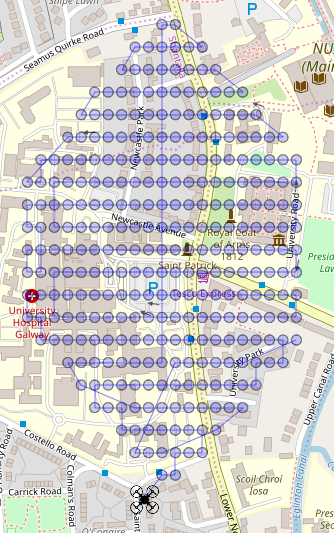
\includegraphics[width=\linewidth, height=72mm]{Chapters/MultiAgentCoverage/MultipleTravellingSalesman/Figs/Hexagon/OneRAV.PNG}
    \end{minipage}
    &
    \begin{itemize}[leftmargin=*]
      \item[] RAV 1 (blue): 7247.2
    \end{itemize}
    \\
    \hline
    %two RAV
    \begin{minipage}[c][74mm][c]{.5\textwidth}
      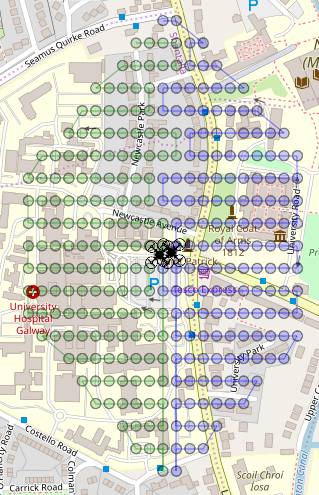
\includegraphics[width=\linewidth, height=72mm]{Chapters/MultiAgentCoverage/MultipleTravellingSalesman/Figs/Hexagon/TwoRAV.PNG}
    \end{minipage}
    &
    \begin{itemize}[leftmargin=*]
        \item[] RAV 1 (blue): 3587.4
        \item[] RAV 2 (green): 3544.2
    \end{itemize}
    \\
    \hline
    
    %three RAV
    \begin{minipage}[c][69mm][c]{.6\textwidth}
      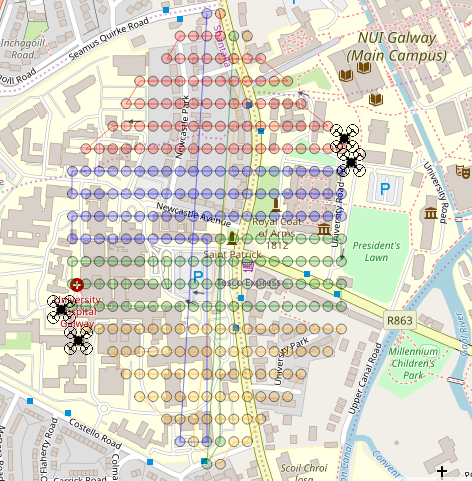
\includegraphics[width=\linewidth, height=67mm]{Chapters/MultiAgentCoverage/MultipleTravellingSalesman/Figs/Hexagon/FourRAV.PNG}
    \end{minipage}
    &
    \begin{itemize}[leftmargin=*]
    \item[] RAV 1 (blue): 2435.6
    \item[] RAV 2 (green): 1629.6
    \item[] RAV 3 (red): 2412.0
    \item[] RAV 4 (yellow): 2245.9
    \end{itemize}
    \\
    \hline
  \end{tabular}
  \caption{Results of applying NN algorithm to a hexagonal region}\label{table:NNAlgoResultsHex}
\end{table}


%\textbf{Irregular Region}
%\\Spacing between grid points: 20m in latitude, 20m in longitude.
%\\Bounding rectangle coordinates: (53.28048,-9.069021), (53.28189,-9.066017), (53.28009,-9.065223), (53.28192,-9.064128), (53.28026,-9.061725), (53.27923,-9.063957), (53.27846,-9.063721), (53.27712,-9.063721), (53.27626,-9.060159), (53.27516,-9.061124), (53.27412,-9.061425), (53.27362,-9.061425), (53.2735,-9.062562), (53.27456,-9.06327), (53.27416,-9.064794), (53.27495,-9.06754), (53.27456,-9.067841), (53.27354,-9.067605), (53.27346,-9.06857), (53.27466,-9.06872), (53.2752,-9.06827), (53.27583,-9.070008), (53.27571,-9.07093), (53.27545,-9.074385), (53.27581,-9.074149), (53.27609,-9.07445), (53.2788,-9.069986), (53.27951,-9.069793), (53.28116,-9.071081), (53.28148,-9.069686)
%\\

%\textbf{Irregular Region}
%\\Spacing between grid points: 20m in latitude, 20m in longitude.
%\\Bounding rectangle coordinates: (53.28048,-9.069021), (53.28189,-9.066017), (53.28009,-9.065223), (53.28192,-9.064128), (53.28026,-9.061725), (53.27923,-9.063957), (53.27846,-9.063721), (53.27712,-9.063721), (53.27626,-9.060159), (53.27516,-9.061124), (53.27412,-9.061425), (53.27362,-9.061425), (53.2735,-9.062562), (53.27456,-9.06327), (53.27416,-9.064794), (53.27495,-9.06754), (53.27456,-9.067841), (53.27354,-9.067605), (53.27346,-9.06857), (53.27466,-9.06872), (53.2752,-9.06827), (53.27583,-9.070008), (53.27571,-9.07093), (53.27545,-9.074385), (53.27581,-9.074149), (53.27609,-9.07445), (53.2788,-9.069986), (53.27951,-9.069793), (53.28116,-9.071081), (53.28148,-9.069686)
%\\

%\begin{table}[H]
%  \centering
%  \begin{tabular}{ | c | m{5cm} | }
%    \hline
%    Planned RAV Routes & Route Lengths (metres) \\
%    \hline
    
    %single RAV
%    \begin{minipage}[c][68mm][c]{.6\textwidth}
%      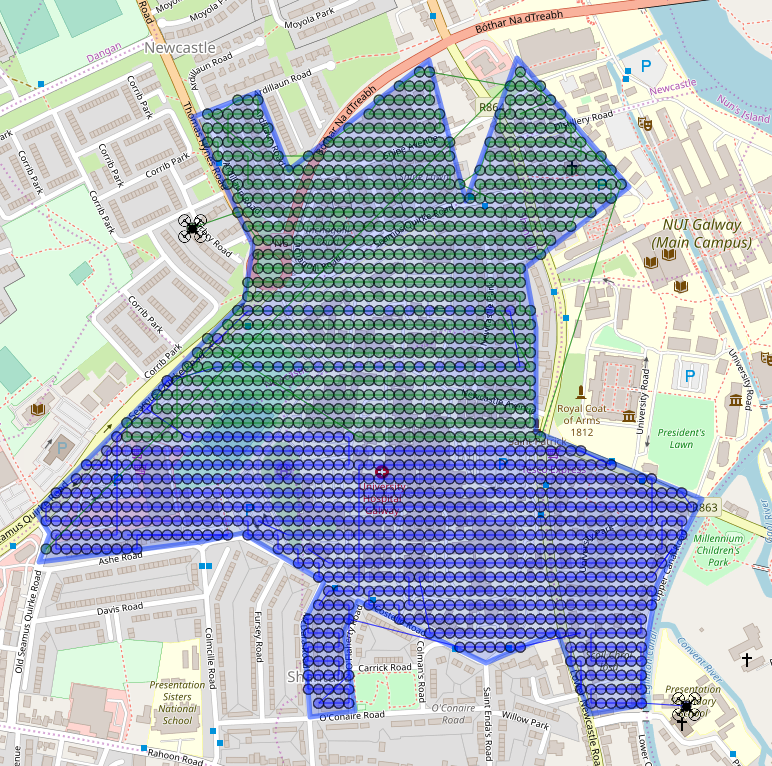
\includegraphics[width=\linewidth, height=66mm]{Chapters/MultiAgentCoverage/MultipleTravellingSalesman/Figs/IrregularRegion/TwoRAV.PNG}
%    \end{minipage}
%    &
%    \begin{itemize}[leftmargin=*]
%       \item[] RAV 1 (blue): 14268.6
%        \item[] RAV 2 (green): 13393.6
%    \end{itemize}
 %   \\
%    \hline
    %two RAV
%    \begin{minipage}[c][68mm][c]{.6\textwidth}
%      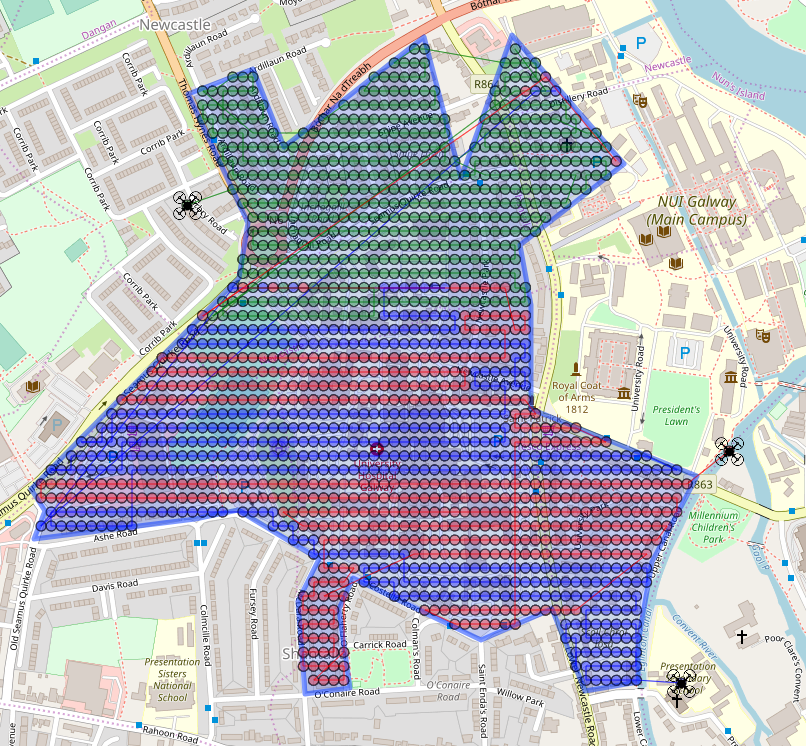
\includegraphics[width=\linewidth, height=66mm]{Chapters/MultiAgentCoverage/MultipleTravellingSalesman/Figs/IrregularRegion/ThreeRAV.PNG}
%    \end{minipage}
%    &
%    \begin{itemize}[leftmargin=*]
%        \item[] RAV 1 (blue): 8879.8
%        \item[] RAV 2 (green): 9596.4
%        \item[] RAV 3 (green): 9433.4
%    \end{itemize}
%    \\
%    \hline
    
    %three RAV
%    \begin{minipage}[c][68mm][c]{.6\textwidth}
%      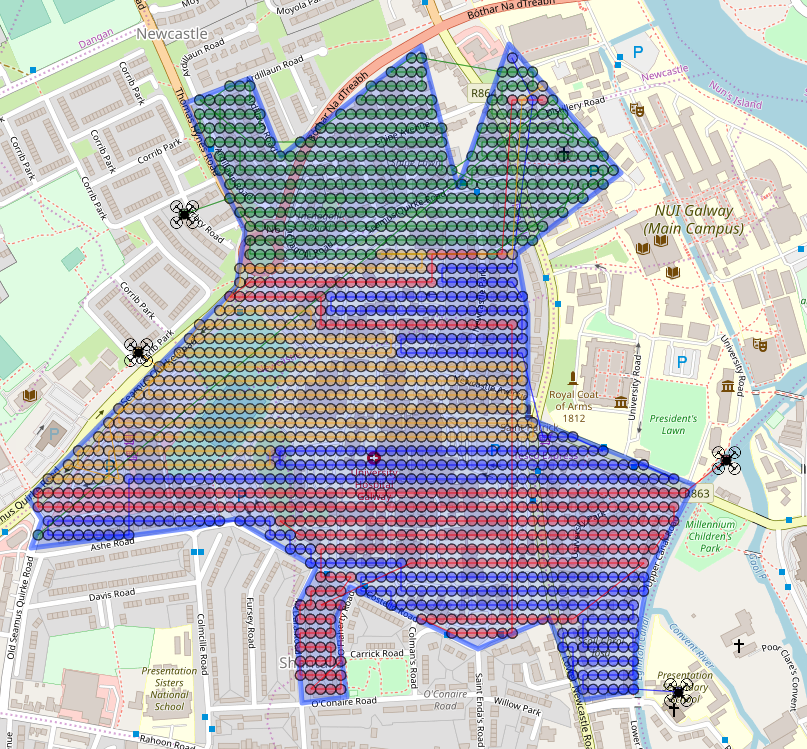
\includegraphics[width=\linewidth, height=66mm]{Chapters/MultiAgentCoverage/MultipleTravellingSalesman/Figs/IrregularRegion/FourRAVSecondAttempt.PNG}
%    \end{minipage}
%    &
%    \begin{itemize}[leftmargin=*]
%    \item[] RAV 1 (blue): 7673.2
%%    \item[] RAV 2 (green): 6354.0
 %   \item[] RAV 3 (red): 6860.6
%    \item[] RAV 4 (yellow): 6368.8
%    \end{itemize}
%    \\
%    \hline
%  \end{tabular}
%  \caption{Results of applying NN algorithm to an irregular region}\label{table:NNAlgoResultsIrregular}
%\end{table}
%\pagebreak



































%\subsubsection{Proof of Lower Bound of Nearest Neighbor Solution}
%Let O be a tour that is an optimal solution to the Travelling Salesperson Problem (TSP) for  a graph G(V, E), where E $\subseteq$ V $\times$ V, with a cost function c$(p_i, p_j)$ defined for all $(p_i, p_j)$ $\in$ E and an induced cost function 
%C($T$) = $\sum\limits_{(p_i, p_j)\in }$C$(p_i, p_j)$ defined for any tour $T$ of G.
%The optimal tour O is an ordered tuple (($p_i, p_j$), ($p_j, p_k$),..., ($p_m, p_n$)) $\subseteq$ E which satisfies:
%\[
%Cost(O) =  \min_{e \subseteq E}\sum_{(p_i, p_j) \in e} c(p_i, p_j) 
%\]
%with the constraint that each $p_i \in$ V must be visited exactly once. This means that O is a Hamiltonian tour of G of minimal cost. 
%\\
%For any partition ($T_1, T_2, ..., T_m$) of an arbitrary tour T', we find:

%\[\text{Cost}(T')=\sum\limits_{k=1}^{m}\sum\limits_{(p_i, p_j)\in T_k} \text{cost}(p_i, p_j) \leq m \times \max_{T_k \in T}
%\sum\limits_{(p_i, p_j)\in T_k}c(p_i, p_j) = 
%m \times \max_{T_k \in T} \text{Cost}(T_k)
%\]

%\noindent Since Cost(O) $\leq$ Cost(T'), for the partition determined by any solution to the TSP, we find that for any solution S to mTSP consisting of the partition ($S_1, S_2, ...,S_m$) for each of the m agents:\\

%\[
%Cost(T)
%\leq Cost(S) \leq  m \times
%\max_{S_k \in S}
%\sum\limits_{(p_i, p_j)\in S_k}C(p_i, p_j)) = Cost of MTS solution, S.
%\]
%This means we can use a solution of the standard Traveling Salesperson problem as a lower bound for comparison with Algorithm \ref{alg:agentRoutesEdited}. For example, the Held-Karp algorithm gives a well-known lower bound when dealing with a metric space \cite{VALENZUELA1997157}.

%We explored a number of solutions to this 



\subsection{Executing Agent Routes in Simulation}
\note{talk about how routes can be executed in sim. env.}
In order to test the algorithms developed in this chapter in a realistic scenario, we utilised the simulation environment described in Chapter \ref{chap:HighFidelitySim}. The AirSim plugin \cite{Shah2017AirSim:Vehicles} provides a straightforward interface to be able to configure the simulation environment to run with a user specified number of UAVs, with an API to send commands to each. We successfully ran a number of tests in simulation using the User Interface to select the bounding area and grid spacing for the UAVs, which interfaced with the code which generated the routes for the UAVs. We then used the AirSim API to send the virtual UAVs to the generated waypoints on each route to gather images. The results of a simulation run showing the executed routes are shown in figure \ref{fig:VirtualPlannedRoutes}


\begin{figure}
    \centering
    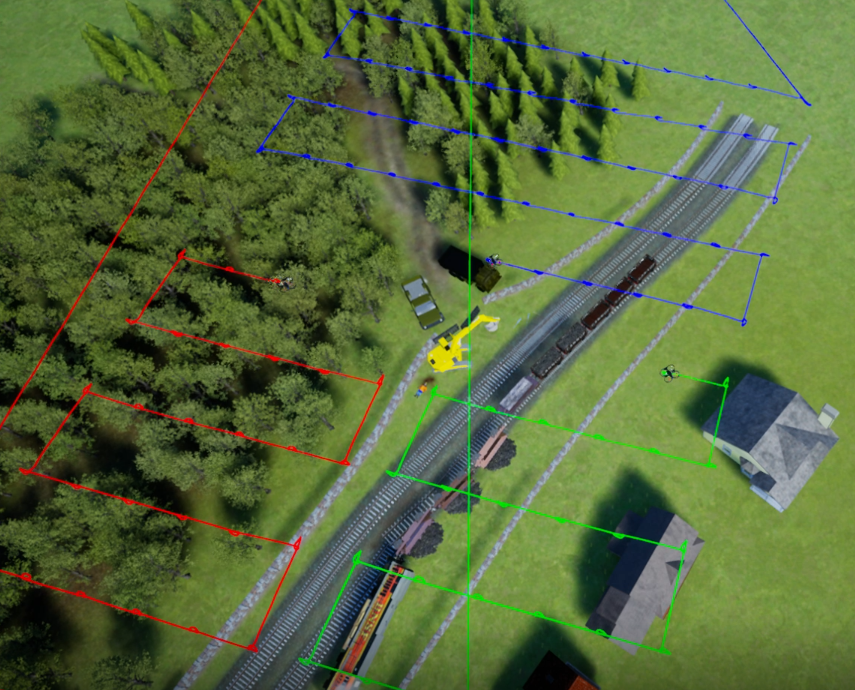
\includegraphics[width=0.6\textwidth]{Chapters/SimulationEnv/Figs/DebuggingLines/RoutesWithRAVsVisible.png}
    \caption{UAVs executing their planned routes in the simulation environment}
    \label{fig:VirtualPlannedRoutes}
\end{figure}

\subsection{Scene Surveying With Battery Constraints and Sampling Times}
Once we had prototyped the NN algorithm in order to find a suitable solution to the simplified problem, we then considered the more general problem, where UAVs have heterogeneous battery constraints, sampling times and 


\note{Keep this very brief - there is not a great research output here. Simply mention that we began looking into using solvers to calculate solutions.}

dsakldfjslkfj

\section{Conclusion and Future Work}
In this chapter we provided the details of how a swarm of UAVs can be used to gather data in a given region described by a polygon. We described how to discretise the region into a set of grid points and we implemented a Nearest Neighbor (NN) heuristic algorithm to generate routes for the swarm of UAVs which visit each grid point in the region exactly once, which is a solution to the multiple Travelling Salesman Problem. For practical purposes in relation to ROCSAFE \cite{rocsafeNUIG}, the project that has funded this work, this solved the surveying problem. The tests carried out in simulation were carried out successfully, using the user interface and custom simulation environment, illustrated in \ref{fig:VirtualPlannedRoutes}, which offers some validation to the work. We then extended this work to use a linear program solver, as proposed in the literature. We managed to prototype a solution using the OR-Tools code repository <provide link>.

Since we were limited by time constraints with this work, we outline some future work that we planned but did not have the time to execute.\par

\subsubsection{Future Work}
We describe some future work that could be done to build on the basic solutions to the problem of finding a scalable solution to the mTSP and VRP described in this chapter. The points outlined are all taken to be specific to the Euclidean grid-based approach that was discussed throughout this chapter.

\begin{enumerate}
    \item The NN solution offered a method that could provide qualitatively good solutions in many scenarios 
    
    \item The quality of the solution to the TSP given by the NN algorithm is known to be dependent on the start position <suitable reference missing>. A common improvement to the algorithm is to run it $n$ times for each possible starting point at each node in the network of $n$ nodes, and then take the best solution found. In the case of the mTSP, for $k$ UAVs, this would mean exploring ${n \choose k}$ different combinations of starting positions, which may make the running time of the algorithm prohibitively long. Therefore, future research could explore an effective way of determining the best starting nodes for the UAVs without implementing a brute force search to improve the NN solution.
    \item Many solutions to the mTSP problem use \textit{iterative improvement} strategies,  which use an existing algorithm to create a solution, then have another algorithm improve the solution.\textit{ Ensemble} strategies are also frequently used, which applies a set of algorithms to the  problem and returns the best solution. The use of either of these techniques with the NN algorithm could provide significantly better results, especially given that this has been shown in the case of Euclidean distance cost functions. For example, reversing some segments that "cross" guarantees an improvement via the \textit{triangle inequality}, as shown in Figure \ref{fig:fixingTourCrossing}. 
    \item Many open-source and commercial linear program solvers exist which are optimized to deal with the mTSP and VRP. We discussed how we used Google's OR-Tools repository <link in footnote> to prototype a solution. Future work could involve optimising the configuration of the problem and choice of back-end solver to produce a scalable solution.
    \item Representing the problem in a different manner may yield a suitable solution that is easier to computer. For example, representing the region to survey as continuous space rather than a discrete grid may facilitate the development of a control algorithm that is simpler and more effective in solving the surveying problem than the ones that exist that deal with discrete grids.
    \item Further theoretical analysis of the algorithm performance could yield insight in how to improve it. Given that it solves some instances of the problem with good results, e.g. that of Figure \ref{table:NNAlgoResultsRect}, the simple, scalable NN solution could be modified to deal with more general problems by using a divide-and-conquer approach to smaller rectangular regions.
    \item UAVs may be unreliable and the assumptions of deterministic sampling times and transition times between locations are not valid in real-world application. A decentralized algorithm which can handle this inherent stochastic element would provide a more robust solution to the surveying problem using multiple UAVs, which could be far superior to the solution presented in this thesis.
    
    
\end{enumerate}


\begin{figure}
\centering
\begin{minipage}{.5\textwidth}
  \centering
  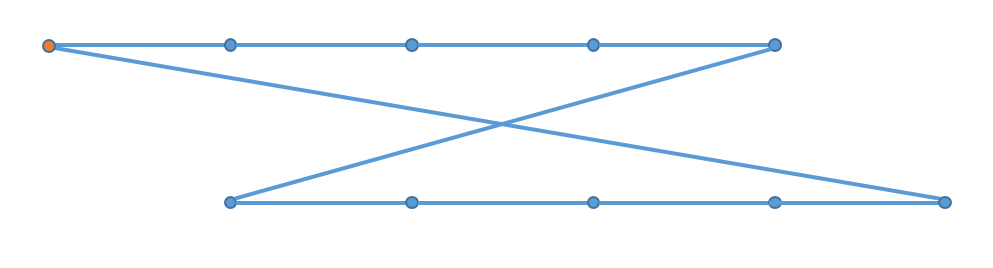
\includegraphics[width=.48\linewidth]{Chapters/MultiAgentCoverage/Figs/crossingSegments.PNG}
  \captionof*{figure}{"X" present in a tour}
  \label{fig:crossingTour}
\end{minipage}%
\begin{minipage}{.5\textwidth}
  \centering
  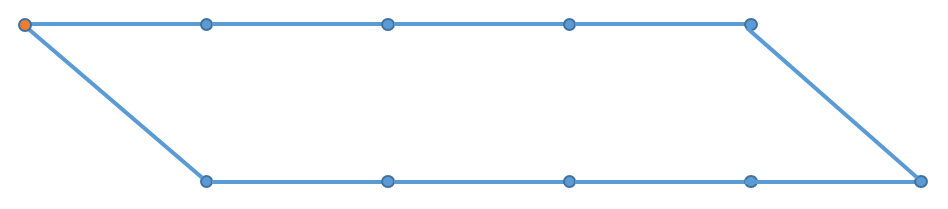
\includegraphics[width=.48\linewidth]{Chapters/MultiAgentCoverage/Figs/nonCrossingSegments.png}
  \captionof*{figure}{"X" removed from tour by reversing segments}
  \label{fig:nonCrossingTour}
\end{minipage}
\caption{Using the triangle inequality to improve tours.}
%Figures based on those found in \href{https://github.com/norvig/pytudes/blob/master/ipynb/TSP.ipynb}{Norvig's TSP github repo.}}
%\footnote{\href {https://github.com/norvig/pytudes/blob/master/ipynb/TSP.ipynb}{https://github.com/norvig/pytudes/blob/master/ipynb/TSP.ipynb}}
\label{fig:fixingTourCrossing}
\end{figure}
%\footnote{\href {https://github.com/norvig/pytudes/blob/master/ipynb/TSP.ipynb}{https://github.com/norvig/pytudes/blob/master/ipynb/TSP.ipynb}}























